\documentclass[12pt,a4paper]{ufpr}

% \usepackage[portuges,brazil]{babel}
% \usepackage[portuguese,brazil]{babel}

\usepackage[english]{babel}
\usepackage[utf8]{inputenc}
\usepackage{amssymb,amsmath,amsfonts}
\usepackage{amsmath}
\usepackage{epsfig}
\usepackage{multirow}

\newcommand{\tuple}[1]{\ensuremath{\left \langle #1 \right \rangle }}
\newcommand{\code}[1]{\textbf{#1}}

\usepackage{ifthen,graphicx,color}

\usepackage{verbatim}
%\usepackage[pdfborder={0 0 0},plainpages=false]{hyperref}

\usepackage[ruled, vlined]{algorithm2e}
\usepackage{listings}
\usepackage{minted}
%\usemintedstyle{trac}

%\usepackage{isolatin1}
\usepackage{amssymb}
\usepackage{subfigure}
\usepackage{caption2}
\usepackage{setspace}
\usepackage{ps-macros}
% \usepackage{psfig}

\usepackage{indentfirst}
%\usepackage[noend]{algpseudocode}
\usepackage{algpseudocode}
\newcommand*\Let[2]{\State #1 $\gets$ #2}
\algrenewcommand\algorithmicrequire{\textbf{Precondition:}}
\algrenewcommand\algorithmicensure{\textbf{Postcondition:}}

\setcounter{secnumdepth}{3}    % n - numero de niveis de subsubsection numeradas
\setcounter{tocdepth}{3}       % coloca ate o nivel n no sumario

\title{KonfigJob: A framework based in bacteriological algorithm for Hadoop
job configuration}
\author{Tiago Rodrigo Kepe}
\advisortitle{Advisor} % ou Orientador
\advisorname{Prof. Dr. Eduardo C. de Almeida}
\advisorplace{Informatics Department, Federal University of Paran�, Brazil}
\city{Curitiba}
\year{2013}

\banca        % nao insira o nome do orientador, ja eh feito automaticamente
{Prof. Dr. Marcos D. Del Fabro}{Informatics Department, Federal University of Paran�}
{Prof. Dr. Gerson Suny�}{Informatics Department, INRIA - University of Nantes, France}
{}{}
{}{}    % se houver um quarto membro na banca, inserir nome e instituicao

\defesa{04 de outubro de 2000} % dia em que foi realizada a defesa da dissertacao


\begin{document}

\makecapaproposta             % cria capa para proposta%
%makecapadissertacao           % cria capa para dissertacao de mestrado %
%makerosto                     % cria folha de rosto para versao final da UFPR %
%\maketermo                     % cria folha com o termo de aprovacao da dissertacao%

%\singlespacing           % espacamento 1 - capa UFPR%
%\onehalfspacing          % espacamento 1/2 %
\doublespacing            % espacamento 2 - UFPR %

\pagestyle{headings}
\pagenumbering{roman}

%\chapter*{Agradecimentos}
%\input{agradecimentos.tex}          % possiu somente o texto

\tableofcontents

%\listoffigures         % se houver mais do que 3 figuras
%\addcontentsline{toc}{chapter}{\MakeUppercase{Lista de Figuras}}
%\newpage

%\listoftables        % se houver mais do que 3 tabelas
%\addcontentsline{toc}{chapter}{\MakeUppercase{Lista de Tabelas}}
%\newpage

\chapter*{Resumo}
\addcontentsline{toc}{chapter}{\MakeUppercase{Resumo}}
Texto do resumo....
           % somente o texto
\newpage

\chapter*{Abstract}
\addcontentsline{toc}{chapter}{\MakeUppercase{Abstract}}
% abstract
Currently with the popularity of internet and phenomenon of the social
networks a large amount of data is generated day-to-day. MapReduce appears as a
powerful paradigm to analyse and process such amount of data. The Hadoop framework
implements the MapReduce paradigm, in which a simple interface is available to
implement MapReduce(MR) jobs. However, in MR jobs developers are allowed to setup several
parameters to draw optimal performance from the available resources, but find a
good configuration is time consuming and a configuration found in an execution
may be impracticable for the next time.

In order to facilitate and automate tuning hadoop jobs, we propose a self-tuning
based on data sampling. Our approach allows to find a good job configuration considering
the data stored and the job in question. The users till can provide their usual
job configurations then get the new job configuration that will be more appropriate
with the current state of data stored and the hadoop cluster. So the users have
end-to-end tool to automate the choice of knobs for each job.
        % somente o texto
\newpage


\pagenumbering{arabic}

\chapter{Introduction} % (fold)
\label{cha:introduction}

\section{Motivation}

MapReduce~\cite{Dean:2004} became the industry de facto standard for parallel processing. Attractive features such as scalability and reliability motivate many large companies such as Facebook, Google, Yahoo and research institutes to adopt this new programming paradigm. 
These organizations rely on Hadoop~\cite{White:2009}, an open-source implementation of MapReduce, to process their information.
Besides Hadoop, several other implementations are available: Greenplum MapReduce~\cite{Greenplum:2008}, Aster Data~\cite{Aster:2011}, Nokia Disco~\cite{Mundkur:2011},  Microsoft Dryad~\cite{Isard:2007}, among others. 

MapReduce has a simplified programming model, where data processing algorithms are implemented as instances of two higher-order functions: Map and Reduce. All complex issues related to distributed processing, such as scalability, data distribution and reconciliation, concurrence, fault tolerance, etc., are managed by the framework. 
The main complexity that is left to the developer of a MapReduce-based application (also called a job) lies in the design decisions made to split the application specific algorithm into two higher-order functions. Even if some decisions may result in a functionally correct application, bad design choices might also lead to poor resource usage.

%%%%%%%%%%%%%%%%%%%% Reescrever este paragrafo
As for any other piece of software, testing may be used to evaluate the quality of MapReduce jobs. The efficiency of testing to detect quality issues in the jobs is in turn directly related to the quality of the test suite. MapReduce jobs work with large amounts of data, which is a major difficulty to generate relevant test data that can reveal quality issues. If on one hand using large data sets as input data is not scalable, on the other hand a small amount of data may not expose errors related to the large-scale aspects: efficient resource usage, correct merge of data, etc.

\section{Contribution}

We present an original approach for the generation of test data that target resource usage defects in MapReduce jobs. We use an evolutionary algorithm to generate test data and propose semantic mutation operators to evaluate the quality of the data with respect to their ability at detecting issues in the design of the map and reduce functions. This focus on testing design decisions lies on two observations. First, these design decisions are essential to implement MapReduce jobs, and they should be systematically tested along with the functionality of the job. Second, the functionality of map and reduce is usually simple (small functions, simple control and data flow) since most of the complexity of these jobs (distribution, synchronization, etc.) is handled by the framework. Consequently, simple test cases tend to cover 100\% of the job under test, can be good at detecting algorithmic errors, but are not sufficient to test the efficiency of the map and reduce design. 

The work presented here contributes to the establishment of systematics testing techniques for MapReduce jobs, through the following proposals:
\begin{itemize}
	\item fault models that focus on design issues when splitting a task between map and reduce functions
	\item an automatic search-based technique to generate test data which target these faults
	\item a series of initial experiments that illustrate the difficulty of detecting these faults, and the capacity of our algorithm at generating data that target them
\end{itemize} 

\section{Outline}

\begin{itemize}
	\item Chapter \ref{cha:background} introduces the  fundamental concepts of the MapReduce framework.
	\item Chapter \ref{cha:testgen} introduces two test quality assessment methods, describes methods to data test generation and 
	      meta-heuristic search methods. Two data test generators are presented with their results.
	\item Chapter \ref{cha:proposal} presents our approach to test data generation for testing MapReduce systems.
	\item In chapter \ref{cha:experiments} we and discuss a case study performed with our solution.
	\item In chapter \ref{cha:conclusion} we conclude our results.
\end{itemize}

%The next section introduces the  fundamental concepts of the MapReduce framework and briefly describes different testing scenarios for MapReduce applications. Chapter~\ref{cha:proposal} introduces two test quality assessment methods, describes methods to data test generation and meta-heuristic search methods. Two data test generators are presented with their results.
%Chapter~\ref{cha:related} discusses related work. 
%Chapter~\ref{cha:conclusion} concludes.

% chapter introduction (end)

\chapter{Key-value model, MapReduce and Hadoop} % (fold)
\label{cha:background}

This chapter introduces some concepts that are used in the subsequent sections:
the key-value model, MapReduce paradigm and Hadoop framework.

\section{Key-value model}\label{section:mapreduce}

Key-value model is a simplified model for data storage. It is based on one linked
pair: the key and the value. Generally, the pair is stored without any aggregation or
creation of data schema, thus all detailing of data is done in runtime. Unlike
other models, such as the relational model~\cite{codd:1970}, in which the simplistic
notion of relation already gives some sense for the data, similarly to the hierarchical
data model~\cite{silber:2005} in which the links that connect the records give
details for the data.

The Data Warehouse(DW) was create to solve some particularities involving relational
model. It is a repository that aggregates data from several sources ~\cite{silber:2005},
through the Extract Transform Load(\textbf{ETL}) technique: data is extracted from
sources, transformed and load in the DW.

Due to the simple storage of the key-value model, data \textit{transformation}
is done in the last phase, so the transformation occurs after the data has been
loaded into the target database. Thus there is a inversion of ETL to ELT(Extract Load Transform).
This inversion cause one issue to process large amounts of data, requiring much
computing power while querying the data. One programming paradigm that handles the
key-value model is the MR that is presented in the next section.

\section{MapReduce}\label{section:mapreduce}
MapReduce is a programming system that allows many processes of one
database to be written in simple way,~\cite{molina:2009}. Vast amount of data
is splitted and assigned to a set of computers, called computers cluster to improve
performance through parallelism. The goal is to omit all complexity for that users
focus on the main problem that is the data processing.

The paradigm is inspired on the high-level \textbf{Map} and \textbf{Reduce} primitives
from functional programming languages. Hence the programmers can focus only on the
creation of the two higher-order functions to solve a specific problem and to generate
the necessary data.

Acording \cite{dean:2008}: [\textit{"the computation takes a set of input key/value pairs,
and produces a set of output key/value pairs."}]. An user writes the map function
that receives a set of key/value pairs and produces an \textit{intermidiate}
set of key/value pairs. The reduce function receives the intermidiate pairs as
input and produces the \textit{resultant} set of key/value pairs. This process is
shown in Figure~\ref{fig:mapReduce}:

\begin{figure}[htbp]
	\centering
	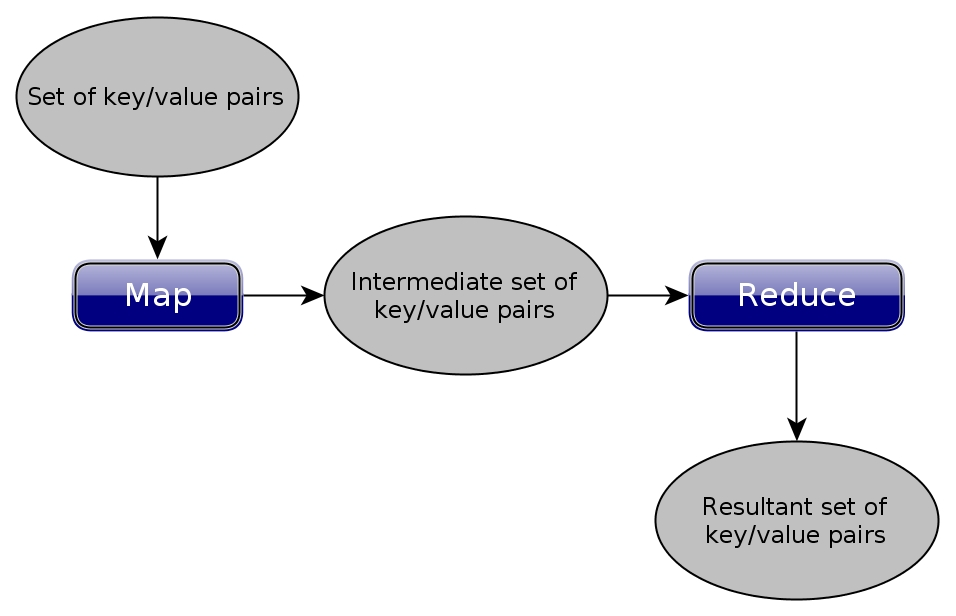
\includegraphics[width=\columnwidth]{img/mapReduce.jpg}
	\caption{Map and Reduce process.}\label{fig:mapReduce}
\end{figure}

\section{Hadoop}
Map and reduce functions are present in Lisp and others functional languages. Recently
the MapReduce paradigm have been implemented by several frameworks such as Greenplum
MapReduce~\cite{Greenplum:2008}, Aster Data~\cite{Aster:2011}, Nokia
Disco~\cite{Mundkur:2011}, Microsoft Dryad~\cite{Isard:2007}, and the one
open-source implemantation from Apache: Hadoop~\cite{hadoop}.

The Hadoop is a framework for reliable, scalable and distributed computing. It provide
an interface to implement the map and reduce functions in high-level which are internally
called as map and reduce tasks. It was designed for users focus on the implementation
those functions, without worrying about the issues involving the distributed computing.
All aspects involving the distributed computing and storage are left to the framework
such as split files, replication, fault tolerance and distribuition of the tasks.

There are two main components on Hadoop:
\begin{itemize}
	\item Hadoop Distributed File System(HDFS);
	\item Engine of MapReduce.
\end{itemize}

The HDFS stores all files in blocks, the block size is configurable per file, all
blocks of one file have the same block size except the last block. It is divided
in two components the \textit{NameNode} and \textit{DataNode}. The NameNode is placed
in one master machine, it stores all metedata and manages all DataNodes. The DataNode
stores data, when one DataNode starts it connects to theNameNode, then responds
to requests from the NameNode for filesystem operations.

The engine of MapReduce is responsible for parallel processing. It is constituted
by one master machine and slave machines, also called workers. The master
designates which slaves will receive map and reduce tasks with its respective input
blocks. The worker that receives map task is called mapper and the slave that receives
reduce task is called reducer.

\subsection{Job processing}

A job is a program in a high-level language(java, ruby or python) that implements
so the map and reduce functions. Initially the master machine receives jobs with
the relative input directory in the HDFS where are all files to be processed (inserted
previously in the HDFS). Then the master requests to the NameNode infomation
about the blocks and file locations, after that it deploys copies of the job across
several workers.

With the blocks information the map task is scheduled to a set of workers
with its respective input blocks. So the mappers process each input blocks, 
generate key/value intermediate pairs and append its in intermediate files. When
the mapper instance terminate it notifies the master. The master split the intermediate
files in blocks and shuffled them to the reducers to process. When all reducers
intances terminate processing, they append their result to the final output file.
The data flow between mappers and reducers are shown in Figure~\ref{fig:mrexecute}.

%%Fazer uma nova figura demonstrando o que foi escrito acima
\begin{figure}[htbp]
	\centering
	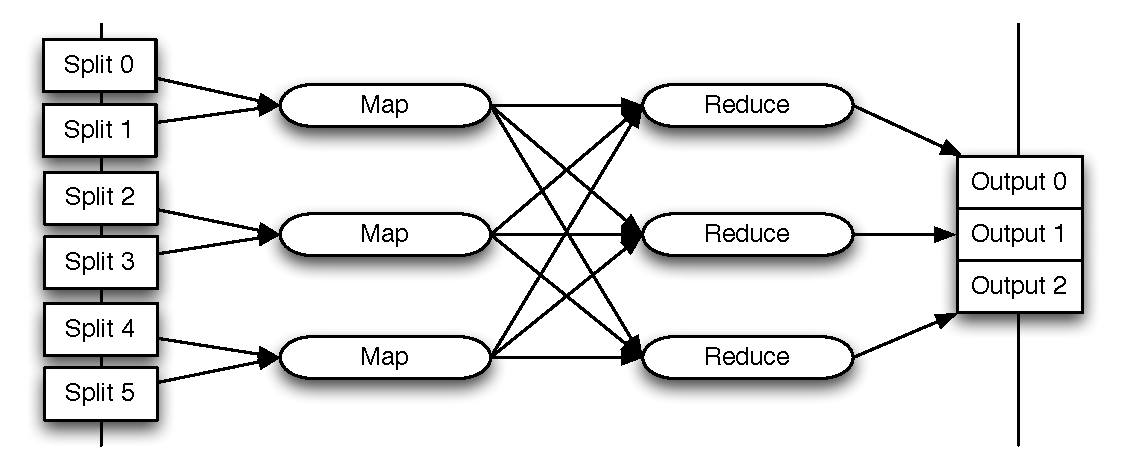
\includegraphics[width=\columnwidth]{img/mapreduce-en.pdf}
%    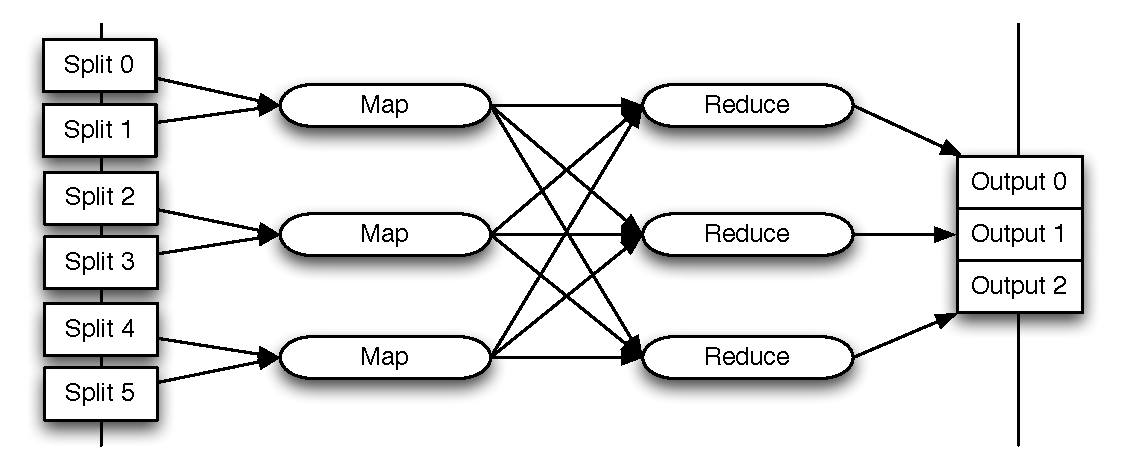
\includegraphics[bb=0 0 1280 960]{img/mapreduce-en.pdf}
	\caption{Execution of Map and Reduce operations}\label{fig:mrexecute}
\end{figure}

\subsection{MapReduce programing}

The whole processing is based on \tuple{key,value} pairs. The mappers receive the
file blocks, the mappers call the map function and pass the line number as key and
the line as the value, so the pair "line number/line content" is the \tuple{k1,v1}.
The map generate the intermediate result set of key and values \tuple{set(k2,v2)}, 
when the mappers finished all values for \textit{k2} are agrouped in a list and
the respective pair \tuple{k2, list(v2)} is generated. This pairs are sorted and
pass as input for reducers that generate the result set:

\begin{center}
\begin{tabular}{c c c c}
	\hline
	   map & $k1,v1$ & $\rightarrow$  & $set(k2, v2)$ \\
	   reduce & $k2, list(v2)$ & $\rightarrow$ & $set(v2)$ \\
	\hline
\end{tabular}
\end{center}

Eventually, when the map result are already available in memory, a local reduce
function \emph{Combiner} is used for optimization reasons, then all values for
determinated key are combined, resulting in a local set \tuple{k2, list(v2)}.
This function runs after the Map and before the Reduce functions on
every node that run map functions. The Combiner may be seen as a \emph{mini-reduce}
function, which operates only on data generated by one machine.

A good example of a MapReduce job is the Grep application listing~\ref{listing:mapper},
which receives as an input several textual documents and as an output a set of pairs
\tuple{Key,Value}, where each key is a different pattern found and the value is the
number of occurrences of the pattern in the files. The responsibility of the Mapper
is to find pattern in the files and the reduce is to sum the amount found each patterns.

The \code{map()} method has four parameters: \code{key}, which is never used; \code{value},
one line that contains the text to be processed; the \code{output}, which will receive
the output pairs and \code{reporter} for debug. The body of the method uses the class
\code{Pattern} to describe a desired pattern, the class \code{Matcher} to find this
pattern, when pattern are found the pair \tuple{matching, 1} is emited to
output.

\singlespacing
\begin{listing}[H]
\begin{minted}[frame=lines,framesep=2mm,fontfamily=courier,fontsize=\scriptsize]{java}
public class RegexMapper<K> extends MapReduceBase
			implements Mapper<K, Text, Text, LongWritable> {

    private Pattern pattern;
    private int group;

    public void configure(JobConf job)
    {
        pattern = Pattern.compile(job.get("mapred.mapper.regex"));
    }

    public void map(K key, Text value, OutputCollector<Text, LongWritable> output,
					Reporter reporter) throws IOException {
        String text = value.toString();
        Matcher matcher = pattern.matcher(text);
        while (matcher.find())
        {
            output.collect(new Text(matcher.group()), new LongWritable(1));
        }
    }
}
\end{minted}
\caption{Class RegexMapper packed in Hadoop~\cite{hadoop}} 
\label{listing:mapper}
\end{listing}

\doublespacing
The implementation of the reduce function is presented in Listing~\ref{listing:reducer}.
The \code{reduce()} method has also four parameters: \code{key}, which contains
a single matching string; \code{values}, a set containing all values associated
to the key (i.e. the matching); \code{output pair}, the resultant pair \tuple{matching,
total} and \code{reporter} for debug. The behavior of the method is straightforward,
it sums all values associated to the key and then writes a pair containing the same
key and the total of matching found.
\singlespacing
\begin{listing}[H]
\begin{minted}[frame=lines,framesep=2mm,fontfamily=courier,fontsize=\scriptsize]{java}
public class LongSumReducer<K> extends MapReduceBase
			 implements Reducer<K, LongWritable, K, LongWritable> {

    public void reduce(K key, Iterator<LongWritable> values,
                     OutputCollector<K, LongWritable> output, Reporter reporter)
                throws IOException {

    // sum all values for this key
    long sum = 0;
    while (values.hasNext())
    {
        sum += values.next().get();
    }

    // output sum
    output.collect(key, new LongWritable(sum));
  }

}
\end{minted}
\caption{Class LongSumReducer packed in Hadoop~\cite{hadoop}} 
\label{listing:reducer}
\end{listing}

\doublespacing
An example of the inputs and the outputs of both functions when applied to a
simple sentence is presented in Table~\ref{table:regexp}. We applied the following
regular expression: \\ \code{"[a-z]$*$o[a-z]$*$"}, this expression find the words that
contains the vowel \code{o} in the midle of them.

\begin{table}[H]
	\begin{center}
	\begin{tabular}{c p{.4\columnwidth} c p{.3\columnwidth} }
		\hline
		map & "Test for hadoop regular expression inside hadoop" & $\rightarrow$ & \tuple{for,1},\tuple{hadoop,1}, \tuple{expression,1}, \tuple{hadoop,1} \\
		reduce & \tuple{for,\{1\}}, \tuple{hadoop,\{1,1\}}, \tuple{expression,\{1\}} & $\rightarrow$ & \tuple{for,1},\tuple{hadoop,2}, \tuple{expression,1}\\
		\hline
	\end{tabular}
	\end{center}
	\caption{Regular expression example}
	\label{table:regexp}
\end{table}

% chapter chapter_name (end)

\chapter{Algorithm for test}
\label{cha:bacAlg}

In this chapter we present the bacteriological algorithm, used to generate and
select the job configurations on Hadoop. 

\section{Genetic Algorithm}
\label{subsec:evolutionay_algorithms}
Evolutionary Algorithms are the technique inspired on biological evolution process,
it aims to select the best inviduals that adapt themselves in the environment. For
this adptation is used biological mechanisms such as \textbf{reproduction}, \textbf{mutation},
\textbf{recombination or crossover} and \textbf{selection}. One the most known
evolutionary algorithms is the Genetic Algorithm, it is closely related to evolution
process.

The Genetic Algorithm work on the gene level, so all changes are done in this level.
Although the gene seem to be one component without much relevance, but changes done
its can be crucial for adptation in the environment, i.e., the genetic changes
can be crucial to survival of one entire population of individuals or even mean
survival of a species. Rosenzweig~\cite{rosenzweig:1995} cites that in the evolution
process barriers may exist, like geographical barrier retricts gene flow within
a sexually reproducing population and these genes could define the existence another
population.

The Genetic Algorithm process describe in Figure~\ref{fig:ga} has its main strategy
based in tree biological mechanisms: \textbf{reproduction}, \textbf{crossover}
and \textbf{mutation} which are further detailed below:

\begin{itemize}
	\item \textbf{Reproduction}: copies the individuals to participe of the next
	stage (the crossover), they are chosen as their abilities in adapt themselves
	in the environment, those abilities can be calculated according with a function
	\textit{F(x)} that is called as the fitness of the individual like described
	in Figure~\ref{fig:ga}. The copy ratio of the individual is based in your fitness,
	the choise is similar spinning a wheel where each invidual receive slots according
	with your fitness. Thus the individual fitness is greater, then your number
	of copies tends to be greater.

	\item \textbf{Crossover}: the crossover is similar the natural process called
	chromosomal crossover, this process is basead on genetic recombination of
	chromosomes	that produce new genetic combinations. Basically the genetic pair
	of two individuals are combined to generate another genetic pair to resultant
	individual, so the new individual has some characteristics of both parent.
	More minutely in the genetic algorithm two individuals are chosen randomly {\bf(A, B)},
	an integer k, between 0 and the size {\it n} of an individual less one, is chosen
	randomly. The new individual {\it A'} is composed by the first {\it k} genes of A
	and the last {\it k - n} genes of B. The individual {\it B'} consists of the
	first {\it k} genes of B and the last {\it k - n} genes of A. 

	\item \textbf{Mutation}: after the crossover stage one mutation occur in the
	genes of new individuals. The process is simple in which one or more genes are
	selected randomly and then are changed (e.g.change one nucleotide of the DNA
	of one chromosome, or one gene is constituted for bits 0 or 1 and one bit is
	changed from 0 to 1).
\end{itemize}

\begin{figure}[htbp]
	\centering
	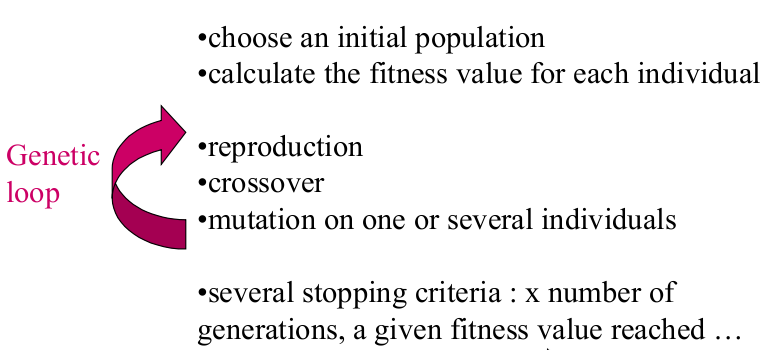
\includegraphics[width=\columnwidth]{img/ga.png}
	\caption{Genetic Algotithm process - Figure extracted of~\cite{baudry}.}\label{fig:ga}
\end{figure}

The algorithm begins with an initial population, for each individual is calculated
your fitness that is the base for reproduction mechanism, so the three biological
mechanisms is called in the specific order already detailed and so the resultant
population is evaluated as one or more criteria, if necessary the three mechanism
are run again and the process continues until the criteria to be achieved.

\section{Bacteriological Algorithm}

Now in the Bacteriological Algorithm(BA) the individual is one bacteria and the focus
of the algorithm is to adapt itself in a given specific environment. The algotithm
is inspired on Genetic Algorithm(GA), but it have some peculiarities that improve
some issues involving the GA and change your behavior.

The BA is more one adaptive approach of GA than one otimization, it introduces a
new mechanism called memorization that is responsable to memorize the best individuals
created along of the generations. As described in ~\cite{baudry} it was proposed
to improve the convergence of the GA, the introduction of the new mechanism might
appear one small modification, but is actually reflect one crucial change of idea
about GA.

Besides of the introduction the new mechanism, the old mechanism crossover was
removed because of the bacteria behavior on its adaptation process in the
environment. This mechanism cannot be used anymore, in terms of natural bacteriologic
process the remotion of the crossover make sense, the bacteria reproduce themself
asexually, the reproduction process consist in duplication of DNA and an after
division to form two new cells.

The algorithm in high-level of abstraction is described in Figure~\ref{fig:ga},
it is fed for one initial population of bacteria, after the bacteriological loop
is started and has four main mechanisms: {\bf Fitness computation}, {\bf Memorization},
{\bf Reproduction} and {\bf Mutation} which are further detailed below:

\begin{itemize}
	\item Fitness computation: the fitness analogously in GA is one way to 	
	differentiate the abilities of each individual in adapt themselves in the
	environment, its calculation depends of one or several criteria defined for 
	the programer and it is used to select the best individuals for the next generation.

	\item Memorization: is the main mechanism introduced by the BA. Its is responsable
	for memorizing the best individuals generated in the process of adaptation,
	as the process continues the population improve more quickly our capacity of
	adaptation. The process consist in memorize the best individuals through of 
	the	generations, if one generation generate bad individuals i.e. generate low
	fitness values, then the memorization operator can ignore this generation and
	use the best individuals already generated in the past to the next generation,
	so avoid regressions in the process.

	\item Reproduction: is similar in GA, the best individuals are sorted ramdomly
	and they are selected to the mutation process. One important point can arise
	in this stage, the population size can grow up exponentially, so thresholds
	must be established.

	\item Mutation: this stage is responsible for generate new individuals, one
	or several genes are changed in order to improve the adaptation of the bacteria
	population in the environment. These new individuals are evaluated by their
	fitness values and they may or may don't be inserted in the set of best
	individuals.

\end{itemize}

\begin{figure}[htbp]
	\centering
	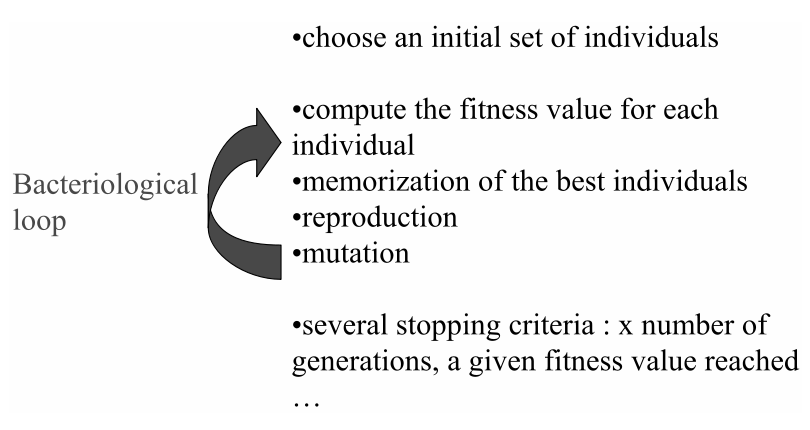
\includegraphics[width=\columnwidth]{img/ba.png}
	\caption{Bacteriological Algotithm process - Figure extracted of~\cite{baudry}.}\label{fig:ba}
\end{figure}


\chapter{Sampling on Hadoop} % (fold)
\label{cha:sample}

In this chapter we present a method for data sampling on Hadoop that is basad
in a random algorithm.

\section{Motivation for sampling}

One important aspect in Big Data environments is the vast amount of data,
that is the main barrier to find a job configuration which best suits to the
current state of the cluster~\cite{Chen:2012}. BAs allow to create new configurations,
but these configurations must be tested in order to select which is the best for
the job at a given moment. Moreover, the volatility of the computing nodes (joining and leaving),
big cluster setups at any time and data volatility, may spoil performance depending
on the configurations setup. 

Therefore, caused by the volatility of the cluster and the data, the job configuration
may become deprecated and needs to be reviewed constantly. The review process consists
in choosing a new configuration and testing it in order to analyse the performance.
But the testing cannot be done on the entire data because may be time consuming.

The main question is: {\it How to test job configurations generated by BAs?} One possible
answer is to run the job on data sampling, because the sampling in a database is
a essential step to improve the response time, moreover run the job on all data
stored would spend a lot of time and also would be impracticable due to larger number
of intermediate configurations generated by the algorithm.

\section{Challenge for data sampling in Big Data environments}

On Big Data environments there are several aspects involving distributed computing
and storage. For data sampling the both aspects are relevants and need to be considered.
In this context, the volume of data is the main issue because the data sampling must
be distributed too, otherwise one machine couldn't bear all data storage in the
cluster then make the data sampling. For instance, suppose that one cluster stores
100 terabytes and we want data sampling of 20$\%$, then each node must sample and
store locally. The resulting sample will be 20 terabytes: which one single machine
may not have such storage capacity.

So the resulting data sample must be distributed in the cluster, because it might
be too big to be store on a single machine. After the sample is obtained, jobs
can be run on the sampling. So, as the example would avoid to run the job on 100
terabytes and run just 20 terabytes.

%So the sampling must be done distributed and it must be done without intrusion
%in the Hadoop, because any change done inside of the framework can propagate collateral
%effects due its complexity. Further more to run test regression is a very costly
%activity~\cite{hadoopUnit} and to create unit test cases for the new changes spend
%much time.

The Hadoop has the structure for distributed computing and storage, so a way to 
produce a sample is to utilize the benefits of Hadoop, i.e. taking into consideration
that the data are already distributed. As a consequence, we can build one MapReduce
program to sample data and then benefit from its advantages.

One of the most used data sample techniques is Random Sampling that consists
in selecting a pre-determined amount of data randomly~\cite{randomsampling}.
In the literature there are several others techniques such as Stratified Random Sampling,
which splits data in strata where each element has the same chance of being selected
\cite{de1986sampling}. Another thechnique is Systematic Sampling that consists
in select randomly one element of the population, from this element the next $k$
elements are select in sequence, the number $k$ may be choosen randomly or based
in some criteria. The systematic process continues till the sample is completed~\cite{systematicsampling}.

%has
%one number {\it k} which is chosen randomly or chosen with some criteria, then
%randomly one element is chosen of the population and from this element till the
%next k-esimo elements in sequence are selected to sample~\cite{systematicsampling}.

In the context of big data there are some implementations of data sample. One example
is MonetDB which is a column-oriented database management system designed to hold
data in main-memory and processing distributed of large-scale data~\cite{monetDB}.
This database supports data sample and uses the {\it Algorithm A} which is based on
a random sample method~\cite{monetDB:sampling}.

The {\it Algorithm A} select {\it n} records from a file containing {\it N} records where
$0\le{\it n}\le{\it N}$. For each record that will be inserted in the sample,
it chooses randomly one number {\it V} that is uniformly distributed between 0 and 1.
Based on {\it V, n} and {\it N}, the number {\it s} is calculated. The set of records
{\it S} is then created from {\it s}. This set contains the {\it (s + 1)} first
records of the file. Then one record is chosen from {\it S} and added to the sample.
The records present in {\it S} are skipped in the next interaction~\cite{vitter:1984}.

The {\it Algorithm A} behaves as the stratified random sampling technique. The creation
of the set S can translate to one stratum that contains neighbors records which one
record is chosen.

Hive is another database management system that performs data sampling based on
random methods. Hive was created to manage the data stored on Hadoop, allowing ad-hoc
queries (with are casts to Hadoop MR jobs), data summarization and analysis of
large datasets. Thus, Hive is considered a DW for Hadoop~\cite{hiveWiki}. It samples at
row or block size level. The row level consists in choosing randomly the rows
according with the colunm name. If the column name is not defined, then the entire row
is selected. If it is defined the choice can be done using the Bucketized Table
in which the sample is done only on the buckets that contains
the specified column~\cite{hiveSample}. The block size sample is also done ramdomly
and consists in selecting the blocks that match with the specified block size.

Those sample methods on Hive are based on random sample and handle structured data.
Hive consists storing the Hadoop data as a data warehouse and facilitate
queries submitted by users. Moreover, the clustering by bucket and block size
requires a prior structuring of data, so in the Hive several information about the
data are previously known.

In Hadoop, data are stored in a unstructured manner and this characteristic is the
biggest challenge to develop data sampling methods. According to~\cite{vitter:1985, cloudera, greg, wikipedia:ReservoirSampling}
the challenge with unstructured data stream can be addressed with Reservoir Sampling:
"{\it Say you have a stream of items of large and unknown length that we can only
iterate over once. Create an algorithm that randomly chooses an item from this
stream such that each item is equally likely to be selected.}"

The Reservoir Sampling algorithm is also a random algorithm. It consists in
randomly choosing {\it k} elements from a list {\it L} containing $N$ items.
The length N is either unknown or too large to fit in memory.

To understand the algorithm one example can clarify the idea. Suppose we have one
reservoir sampling of size equal $1$ and we have to get one item such
that all items have the same probability to be choosen.

In the first round when the first item cames the probability is $P(1)^{1}=1$ because
the stream length is $1$ at the moment and we unknow if the stream finished. When
the next element cames (second element), the first element has been holding and
we need to choose continuing hold the first or choosing the second element. So,
the probability to choose the second element is $P(2)=\frac{1}{2}$ because the stream length
is $2$ at the moment. On the other hand, the probability $P(1)^{2}$ continuing hold the
first element is the probability to choose it in the last round multiple by the
probability doesn't choosing the second element, which is $P(1)^{2}=P(1)^{1} \times \overline{P(2)} = 1 \times \left(1-P(2)\right) = 1 \times \left(1 - \frac{1}{2}\right) = 1 \times \frac{1}{2} = \frac{1}{2}$.
So, the probability of the first and the second element in the second round is $\frac{1}{2}$.

In the next round when the third element cames, we need to decide if continue holding
the element chosen in the last round or if we choose the third element. The probability
to choose the third element is $P(3) = \frac{1}{3}$ because the stream length at the moment
is 3. Now, we need to calculate the probability to continue holding the element
chosen in the last round, considering which is the first element, its probatility
in the third round is the probability of it in the second round multiple
by the probability doesn't choosing the third element: $P(1)^{3}=P(1)^{2}\times\overline{P(3)} = \frac{1}{2} \times \left(1-P(3)\right) = \frac{1}{2} \times \left(1 - \frac{1}{3}\right) = \frac{1}{2} \times \frac{2}{3} = \frac{1}{3}$.
So, the probability of the first, second and third element in the third round is
the same, i.e. $\frac{1}{3}$.

In sequence, for the $Nth$ round the probability of all elements is $1/N$. We
can prove such idea by induction:
\\
\\
\\
\\
\begin{itemize}
	\item \emph{Base Case}: $N = 1$.
		\begin{alignat*}{1}
			\texttt{The probability for the first element is $P(1) = \frac{1}{N} = 1$.}
		\end{alignat*}

	\item \emph{Induction Step}: $N > 1$.\\
		\texttt{By the induction hypothesis, the probability for all elements in the\\
				round $N$: $P(1)$ $...$ $P(N)$ $=$ $\frac{1}{N}$.}\\
		\texttt{In the round $N+1$, when the $N+1$ element cames its probability to be chosen is
				$P(N+1) = \frac{1}{N+1}$. Because the stream length is $N+1$ at the moment.}\\
		\texttt{We need to prove that the probability of the all other elements is the same.}
		\texttt{Let's prove the probability of the elements 1 to N in the round $N+1$:}
		\begin{alignat*}{2}
			\texttt{$P($$1$ $to$ $N)$ = }& \texttt{(the probability of the all elements in the round $N$)}\\
			\texttt{$\times$} 		 & \texttt{(the probability doesn't choose the element $N+1$)} \\
			\texttt{$P($$1$ $to$ $N)$ = }& \texttt{$P(1$ $to$ $N)^{n}$ $\times$ $\overline{P(N+1)}$}\\
			\texttt{$P($$1$ $to$ $N)$ = }& \texttt{$\frac{1}{N}  \times \left(1 - \frac{1}{N+1}\right)$} \\
			\texttt{$P($$1$ $to$ $N)$ = }& \texttt{$\frac{1}{N}  \times \frac{N}{N+1}$}\\
			\texttt{$P($$1$ $to$ $N)$ = }& \texttt{$\frac{1}{N+1}$}
		\end{alignat*}
		\texttt{So, the probability of all elements in the round $N+1$ is $\frac{1}{N+1}$.}\\
		\begin{comment}		
		\begin{flalign*}
			&|\vec a| = \sqrt{3^{2}+1^{2}} = \sqrt{10} & \\
			&|\vec b| = \sqrt{1^{2}+23^{2}} = \sqrt{530} &\\ 
			&\cos v = \frac{26}{\sqrt{10} \cdot \sqrt{530}} &\\
			&v = \cos^{-1} \left(\frac{26}{\sqrt{10} \cdot \sqrt{530}}\right) &\\
		\end{flalign*}
		\end{comment}
\end{itemize}


This prove can be generalized to the reservoir of the length $K$. So, an implementation
of the reservoir algorithm is presented in algorithm~\ref{alg:sample}.
The goal is to build a reservoir which is smaller than the memory. So
it receives as parameter the number $K$ that is the resulting sampling size
and $stream$ of data that constantly receives new data. Initially the resultant
sampling is assigned with the first $K elements$, so the algorithm
aims to calculate the probability of the next element, (e.g. $K+1$), to be inserted
to the sample, which is $P(K+1) = \frac{K}{K+1}$, after one random number ($randNumber$)
between 0 and 1 is chosen, if $randNumber < P(K+1)$, then the next element
is added to random position in the resultant sample.

\begin{algorithm}
		\caption{Algorithm for Reservoir Sampling \label{alg:sample}}

        \SetKwInOut{Input}{Input}
        \SetKwInOut{Output}{Output}
		\Input{$k$ size of sample}
		\Input{$stream$ data stream with indefided length}
        \Output{$arraySample$[$k$]}

		\For{$i = 1 \to k$} {
			$arraySample[i] \leftarrow stream[i]$
		}

		$nextElement \leftarrow k$

		\While{$stream$ != $EOF$} {
			$nextElement \leftarrow nextElement + 1$

            $probability \leftarrow k/nextElement$

			$randNumber \leftarrow Random(0,1)$

			\If {$randNumber < probability$}
			{
                $pos \leftarrow Random(1,k)$

				$arraySample[pos] \leftarrow stream[nextElement]$
			}
		}

        \Return{$arraySample$}
\end{algorithm}


%%%%%%%%%%%%%%%%%Termina frase acima %%%%%%%%

However, choosing the number {\it K} is hard task, because the resultant sample must
be representative and fit in memory. To solve this problem Vitter~\cite{vitter:1985}
suggests to store the reservoir on secundary storage (hard disk). This
approach may be inapplicable for Hadoop, because the secundary storage
is HDFS and the time needed to retrieve the reservoir and update is long, caused
by the communication overload in contact the namenode, look up the reservoir
in the cluster and make the reservoir available for the algorithm in the current
round.

\section{One method for data sampling on Hadoop}

We propose the follow algorithm based on the MR paradigm to generate data
samples on Hadoop. We intend to enjoy the distributed architecture of Hadoop, so
we can classify each line by the mappers and perform the sample distributed using
the reducers. Our approach follows the random algorithm family which has been used
widely in database and big data environments, and it performs the sampling in row
level.

First of all, we present the behavior of the algorithm on map and reduce process
using the Figure~\ref{fig:sampleProcess}. Initially the program receives tree files:
{\it file1, file2 and file3}. There are two mappers to classify each line of the files
and generate the output \tuple{lineNumer, content}. Then, the shuffle step
aggregates each content of the same key:\\
\tuple{lineNumber, \{content1, content2,..., contentN\} }.

The only reducer receives the shuffle output and, for each content of the same key,
chooses one random number. If it is less than sample threshold then chooses this
content, otherwise discards it.

\begin{figure}[htbp]
	\centering
	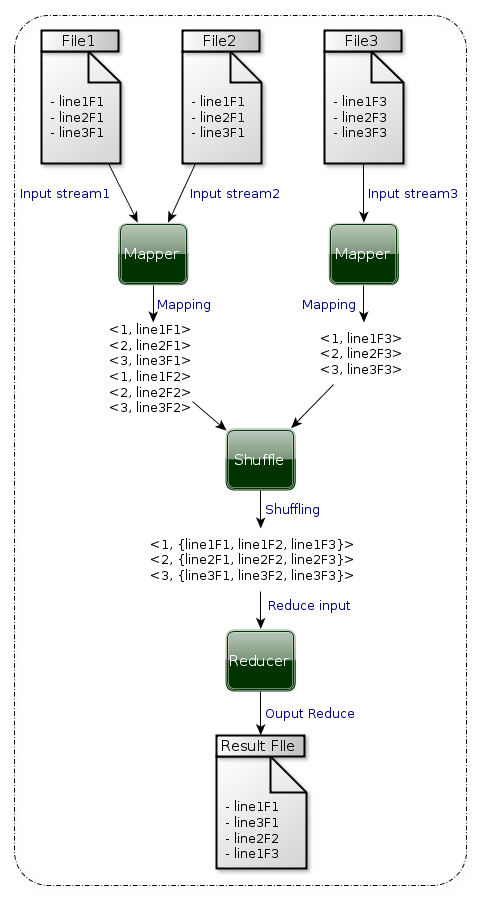
\includegraphics[width=210px,height=400px]{img/sampleProcess.png}
	\caption{Map and Reduce random sample process}\label{fig:sampleProcess}
\end{figure}

The map function is described by algorithm~\ref{alg:map}. Before presenting the
algorithm, some previous definitions are necessary. Let us denote {\it F} the set
of files stored on the cluster, {\it f} a file belonging to {\it F}, {\it l} current
line of {\it f} and {\it o} the order of the {\it L} in {\it F}.

\begin{algorithm}
		\caption{Map function for data sample \label{alg:map}}

        \SetKwInOut{Input}{Input}
        \SetKwInOut{Output}{Output}
		\Input{$F$ file set in the cluster}
        \Output{$map<Integer, String>$ 	resultant list of key-value}

		$map \leftarrow  \{\}$

		\For{\textbf{each} $f \in F$} {

			$l \leftarrow f.getNextLine()$

	    	$o \leftarrow l.getOrder()$ 

			$map.put$($o$, $l$)

		}
		
        \Return{$map$}
\end{algorithm}


The map function consists in classifying each {\it L} in the {\it F} with
it respective order {\it o}. Then intermediate key-value pair \tuple{o, l}
are emitted. Next, each pair is added to a map structure that is the output of
the map function. After the shuffle phase aggregates values sharing the same key.
These aggregated values are the input for reduce function.

\begin{algorithm}
		\caption{Reduce function for data sample \label{alg:reduce}}

        \SetKwInOut{Input}{Input}
        \SetKwInOut{Output}{Output}
		\Input{$mapList<key, values>$ list of key-values aggregated by shuffle phase}
        \Output{$list$ of selected values}

		\For{\textbf{each} $key \in mapList$} {

			\For{\textbf{each} $v \in values$} {
				$rand \leftarrow random(1, n)$

				\If{$rand \leq n$} {
					$list.add(v)$
				}

			}

		}

        \Return{$list$}
\end{algorithm}

The reduce function is in charge of the sampling and is described by algorithm~\ref{alg:reduce}.
Before presenting the algorithm, some previous definitions are necessary. Let us
denote {\it mapList} the intermediate set generated by map phase and aggregated
for the shuffle phase, it contains tuples \tuple{key, list<values>}. The {\it key}
is a key belonging to the {\it mapList}, and {\it values} is a set of values sharing
the same key. The {\it v} is a value belonging to {\it values} and {\it n} is
the amount of the values sharing the same key.

First the reduce algorithm iterates in each {\it key} and get the {\it values}
list. Then for each value {\it v} that share the same key, one random number
between the 1 and {\it n} is chosen. If the random number is lower or equal toz
{\it n} then {\it v} is added to resultant list. 

\chapter{Domain-Specific Language} % (fold)
\label{cha:dsl}

In this chapter we present some fundamentals about Domain-Specific Language~(DSL) and
a language used as interface with the users and self-tuning.

A \textit{DSL} is a way to approach some specific
context through appropriate notations and abstractions~\cite{deursen:2000}. DSL
transforms a particular problem domain into a context intelligible for expert
users that can work in a familiar environment.

Problem domain is a crucial term of DSL that requires prior background of the
developers in the specific context. The developers must be expert in the domain
in order to develop a DSL that cover the features required for the users. There are
a lot of examples of DSLs in differents domains: (LEX, YACC, Make, SQL,
HTML, CSS, LATEX, etc.)~\cite{bentley:1986}.

DLSs normally focus on specific domains, containing notations and specific abstractions.
Also it is a \textit{small} and \textit{declarative} language. A
DSL can be extended to different domains. Such DSL is called general-purpose
language (GPL), because its expressiveness power is not restrict to
an exclusive domain, examples of such DSLs are Cobol and Fortran, which
could be viewed as languages focused on the domain of business and scientific
programming  ~\cite{deursen:2000}.

DSL are used in several areas, such as Software Engineering, 
Artificial Intelligence, Computers Architecture~(in this area a
good exemple is VHSIC Hardware Description Language (VHDL), where VHSIC stand for 
{\bf V}ery {\bf H}igh {\bf S}peed {\bf I}ntegrated {\bf C}ircuits), Database
Systems~(SQL, Datalog, QBE, Bloom), Network~(where its
protocols are examples of DSLs), Distribuited Systems, Multi-Media
and among others. A current area that have been emerged recently is \textbf{Big Data}.
This area may be considered as a sub area of Database, but is has many
particularities that involve a mix features of Database and Distributed Systems.

\section{DSL Design Methodology}

The first step to create a new DSL consists in identifing the problem domain. Depending on
the context, it is not trivial to abstract the complete knowledge of the domain, because
the developers must have a deep prior knowledge of the context, so considering all
variables and intrinsics aspects belonging to the domain. Furthermore, sometimes
the context can cover more than one domain (for example the GPLs). In other cases
the correct abstraction of the domain is fast and there is not room for doubts
and equivocation. In both cases the foreknowledge of the developers is the factor
that influences the most the quality of the resulting DSL.

After identifying the problem domain developers must abstract all relevant 
aspects from it. For example {\it VHDL}, group semantic notations and operations
on logical circuit that allows to express logical components: gates circuits, bus, datapath and
control signals. With these four components we can describe any logical circuit
since a ALU~(Arithmetic Logic Unit), register bank till one complex microprocessor. 

The next step consists in designing a DSL that expresses applications in the domain. DSL
will have limited concepts which are all focused on the specific domain. To
design the DLS, it is necessary to analyse the relationship between it and the existing
languages. According to~\cite{mernik:2005}, there are some design patterns to
develop a DSL based on existing languages that is represented by figure ~\ref{fig:patterns}.

\begin{figure}[htbp]
        \centering
        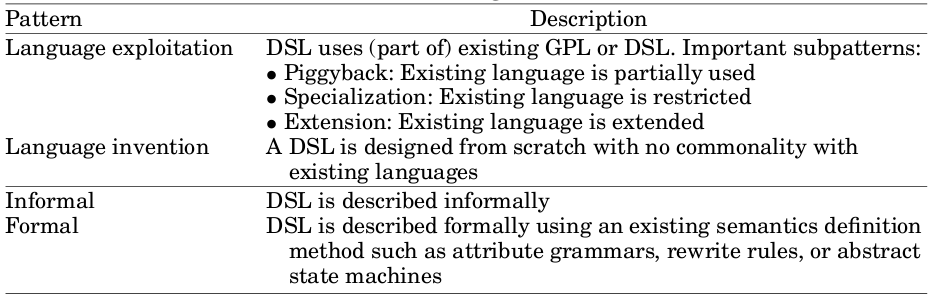
\includegraphics[width=\columnwidth]{img/designPatterns.png}
        \caption{Design patterns - Figure extracted from~\cite{mernik:2005}.}\label{fig:patterns}
\end{figure}

In the implementation, a library with the semantic notations are built
together with a compiler that perfoms the lexical, syntactic and semantic analysis, 
after converting the DSL programs to sequence of library calls. Generally the library
and the compiler are built with support of the tools or framework developed
for this purpose. Xtext~\cite{xtext} and Groovy~\cite{groovyDSL, groovyDSLBook}
are examples of tools to develop DSLs.

\section{Context Transformation}
\label{sec:contextTrans}

Our context is focused on Hadoop environment that have its own particularities. Thus,
a context transformation is mandatory to implement the bacterionlogical algorithm
on such environment.

On Hadoop there is huge set of configuration parameters, we called one specific 
parameter as \textit{knob}. A job use several knobs which we called as set of knobs. 
When sets of knobs are agglomerate we have a population of set of knobs.

In the context tranformation, each component of genetic
context was translated to one component of Hadoop environment. Figure~\ref{fig:transformation}
shows that a gene is transformed into a knob,
an individual (which is a set of genes) is transformed into a set of knobs and,
an individuals population is transformed into a population of set of knobs.

\begin{figure}[htbp]
        \centering
        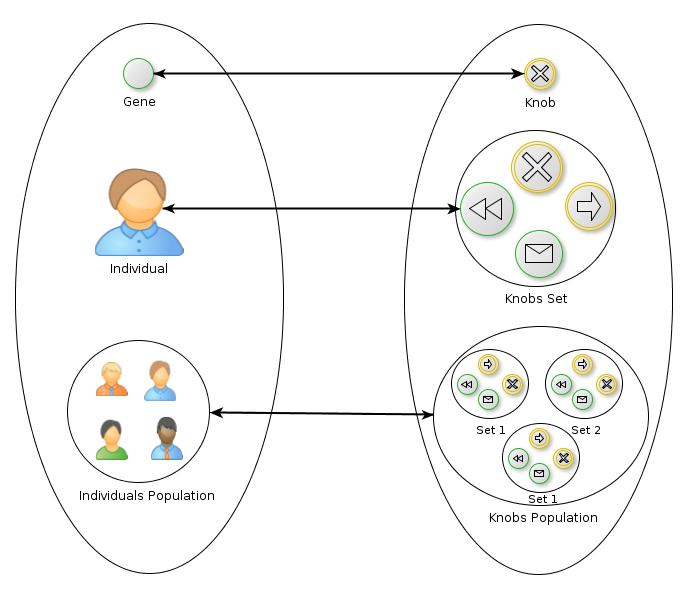
\includegraphics[width=\columnwidth]{img/transformation.jpg}
        \caption{Context transformation.}\label{fig:transformation}
\end{figure}

An interesting characteristic of the tranformation is its bijection that one
component in the genetic domain is translated to one component in Hadoop domain. Beyond
that the transformation has inversion property, i.e, all components in Hadoop domain
can be translated to respective components in genetic domain. That properties
represent compatibility between both domains and somewhat a good representativeness.
\\
\\
\\
\\
\\
\\
\\
%-------------------------------------------------------------------------------
% Put here one formal teorem and a prof for the afirmation above. ^^^^^^^^^^^^^^
%-------------------------------------------------------------------------------
\section{DSL Proposal}

Our DSL proposal is based on the \textbf{Xtext} framework~\cite{xtext}. It requires
to define a grammar and rules for the specific domain. The base of the DLS is the
self-tuning using BA. So our effort aims to describe rules to represent all aspects
and components required for self-tunning.

Our domain has the following components:

\begin{itemize} 
    \item The job with its properties;
    \item The knobs;
    \item The knob with own type, minimum and maximum thresholds and its initial value.
\end{itemize}

Based on these components we present a preliminary version of our DSL:

\singlespacing
\begin{listing}[H]
\begin{minted}[mathescape,frame=lines,framesep=2mm,fontfamily=courier,fontsize=\scriptsize]{python}
DomainModel:
	job=Job;
	
Job:
	'Job' name=ID '{'
        setProperties+=Properties*
		setKnobs+=Knobs*
	'}'
;

Properties:
    'Properties' '{'
        properties+=Property
    '}'

Property:
    name=ID Value
;

Value: String;


Knobs:
	'knobs' '{'
		knobs+=Knob*
	'}' 
;

Knob:
	 name=ID Type
;

Type:
	IntType | FloatType | BoolType
;

IntType:
	'int' MinInt MaxInt '=' INT
;
MaxInt: INT;
MinInt: INT;

FloatType:
	'float' MinFloat MaxFloat '=' Float
;
MaxFloat: Float;
MinFloat: Float;

Float:
	INT*'.'INT*
;

BoolType:
	'boolean' '=' Boolean
;
Boolean:
	'true' | 'false' 
;

\end{minted}
\caption{Initial DSL proposal} 
\label{listing:dlsProposal}
\end{listing}

Oll the rules forming our grammar are presented below:
\begin{enumerate}
	\item
		\singlespacing
		\begin{listing}[H]
		\begin{minted}[mathescape,frame=lines,framesep=2mm,fontfamily=courier,fontsize=\scriptsize]{python}
			DomainModel:
				job=Job;
		\end{minted}
		\label{listing:modelRule}
		\end{listing}

		The first rule in a grammar is always used as the entry or starting rule.
		It espresses that the \textbf{DomainModel} contains one element \textbf{Job}
		assigned to a feature called \textit{job}.

	\item
		\singlespacing
		\begin{listing}[H]
		\begin{minted}[mathescape,frame=lines,framesep=2mm,fontfamily=courier,fontsize=\scriptsize]{python}
			Job:
                'Job' name=ID '{'
                    setProperties+=Properties*
                    setKnobs+=Knobs*
                '}'
            ;	
		\end{minted}
		\label{listing:modelRule}
		\end{listing}

		The rule \textbf{Job} starts with the definition of a keyword ({\it Job})
		followed by a name. Between brackets the job contains one indefinite number
		(*) of \textbf{Properties} and \textbf{Knobs} which will be added (+=) to
        a feature called setProperties and setKnobs, respectively.

    \item
		\singlespacing
		\begin{listing}[H]
		\begin{minted}[mathescape,frame=lines,framesep=2mm,fontfamily=courier,fontsize=\scriptsize]{python}

            Properties:
                'Properties' '{'
                    properties+=Property
                '}'
            ;
		\end{minted}
		\label{listing:modelRule}
		\end{listing}

        The rule {\bf Properties} starts with the definition of a keyword {\bf Properties}
		and between brackets contains one indefinite number (*) of \textbf{Property}
		which will be added~(+=) to a feature called properties.

    \item
		\singlespacing
		\begin{listing}[H]
		\begin{minted}[mathescape,frame=lines,framesep=2mm,fontfamily=courier,fontsize=\scriptsize]{python}

            Property:
                name=ID Value
            ;

            Value: String;
		\end{minted}
		\label{listing:modelRule}
		\end{listing}

        These two rules are used to describe job properties, each property has an
        ID followed by its value. The value is an String.

	\item
		\singlespacing
		\begin{listing}[H]
		\begin{minted}[mathescape,frame=lines,framesep=2mm,fontfamily=courier,fontsize=\scriptsize]{python}
			Knobs:
				'knobs' '{'
					knobs+=Knob*
				'}' 
			;
		\end{minted}
		\label{listing:modelRule}
		\end{listing}

		The rule \textbf{Knobs} starts with the definition of a keyword {\bf knobs}
		and between brackets contains one indefinite number (*) of \textbf{Knob}
		which will be added (+=) to a feature called knobs.

	\item
		\singlespacing
		\begin{listing}[H]
		\begin{minted}[mathescape,frame=lines,framesep=2mm,fontfamily=courier,fontsize=\scriptsize]{python}
			Knob:
				 name=ID Type
			;
		\end{minted}
		\label{listing:modelRule}
		\end{listing}

		The rule \textbf{Knob} contain one name followed by a \textbf{Type} with
		your peculiarities explained below.

	\item
		\singlespacing
		\begin{listing}[H]
		\begin{minted}[mathescape,frame=lines,framesep=2mm,fontfamily=courier,fontsize=\scriptsize]{python}
			Type:
				IntType | FloatType | BoolType
			;
		\end{minted}
		\label{listing:modelRule}
		\end{listing}

		The rule \textbf{Type} can accept three type: \texttt{integer}, \texttt{float} or \texttt{boolean},
		this three are all possibles types on hadoop parameters configuration.

	\item
		\singlespacing
		\begin{listing}[H]
		\begin{minted}[mathescape,frame=lines,framesep=2mm,fontfamily=courier,fontsize=\scriptsize]{python}
			IntType:
				'int' MinInt MaxInt '=' INT
			;
			MaxInt: INT;
			MinInt: INT;
		\end{minted}
		\label{listing:modelRule}
		\end{listing}

		These three rules are used for integer types, the rule \textbf{IntType}
		starts with the keyword {\bf int} followed by your respective minimum
		and maximum possibles values. In sequence there is the keyword {\bf '='}
		and the initial value for the knob.

	\item
		\singlespacing
		\begin{listing}[H]
		\begin{minted}[mathescape,frame=lines,framesep=2mm,fontfamily=courier,fontsize=\scriptsize]{python}
			FloatType:
				'float' MinFloat MaxFloat '=' Float
			;
			MaxFloat: Float;
			MinFloat: Float;

			Float:
				INT*'.'INT*
			;
		\end{minted}
		\label{listing:modelRule}
		\end{listing}

		These four rules are used for float types, the rule \textbf{FloatType} is
		similar the IntType rule, it starts with the keyword {\bf float} followed
		by your respective minimum and maximum possibles values. In sequence there
		is the keyword {\bf '='} and the initial float value for the knob. The rule
		{\bf FloatType} expresses the float format.

	\item
		\singlespacing
		\begin{listing}[H]
		\begin{minted}[mathescape,frame=lines,framesep=2mm,fontfamily=courier,fontsize=\scriptsize]{python}
			BoolType:
				'boolean' '=' Boolean
			;
			Boolean:
				'true' | 'false' 
			;
		\end{minted}
		\label{listing:modelRule}
		\end{listing}

		The last rule {\bf BoolType} expresses the boolean type, it starts with
		the keyword {\bf boolean} followed by signal of \textbf{'='} and the initial
		boolean	value that can be {\bf true} or {\bf false}.

\end{enumerate}

%\input{capitulo4.tex}
%\input{capitulo5.tex}
%\input{capitulo6.tex}
%\input{anexo1.tex}     % se houver anexo



\bibliographystyle{brazil}
\bibliography{kepe}
% utilize macros (3 primeiras letras do mes em ingles, minusculas) no seu
% .bib para atribuir o nome do mes em portugues nas referencia,
% se o style for brazil, outros estilos tambem aceitam estas macros
% Ex:
%
% @InProceedings{teste,
%   author =       {Luciano}
%   year =         {2000}
%   month =        {}#sep;
% }
%
\addcontentsline{toc}{chapter}{\MakeUppercase{Bibliografia}}

\singlespacing
\makecapadissertacao

\end{document}
